\documentclass[letterpaper,titlepage,12pt]{report}
\usepackage[latin1]{inputenc}
\usepackage[spanish]{babel}
\usepackage[pdftex]{graphicx}
\usepackage{graphicx}
\usepackage{float}
\usepackage{amssymb,amsfonts,amsmath,latexsym,theorem}
\usepackage{amsfonts}
\usepackage{tabularx}
\usepackage[usenames]{color}
\usepackage[table,xcdraw]{xcolor}

\newtheorem{definition}{Definici\'on}
\newtheorem{theorem}{Teorema}
\newtheorem{Example}{Ejemplo}
\newtheorem{Exercise}{Ejercicio}
\newtheorem{proposition}{Proposici\'on}
\newtheorem{lemma}[theorem]{Lema}
\newenvironment{proof}[1][Demostraci\'on]{\textbf{#1.} }{\rule{0.1cm}{0.1cm}}
\newtheorem{remark}{Obsevaci\'on}
\newtheorem{example}[theorem]{Ejemplo}
\newtheorem{corollary}{Corolario}
\usepackage[none]{hyphenat} %evitar malos cortes de silabas

\begin{document}
\sloppy %evitar malos cortes de silabas

\subsubsection{Ejemplo en \'epoca de sue\~no MOR}

Para tener una ida m\'as clara de lo que se esta realizando con el m\'etodo DFA, se considera una \'epoca de sue\~no MOR cualquiera, la cual consta de 30 segundos, con una frecuencia de 512 Hz, teniendo un total de 15,360 puntos. Representados en el siguiente gr\'afico \ref{ejemplo}.  

\begin{figure}[H]
\begin{center}
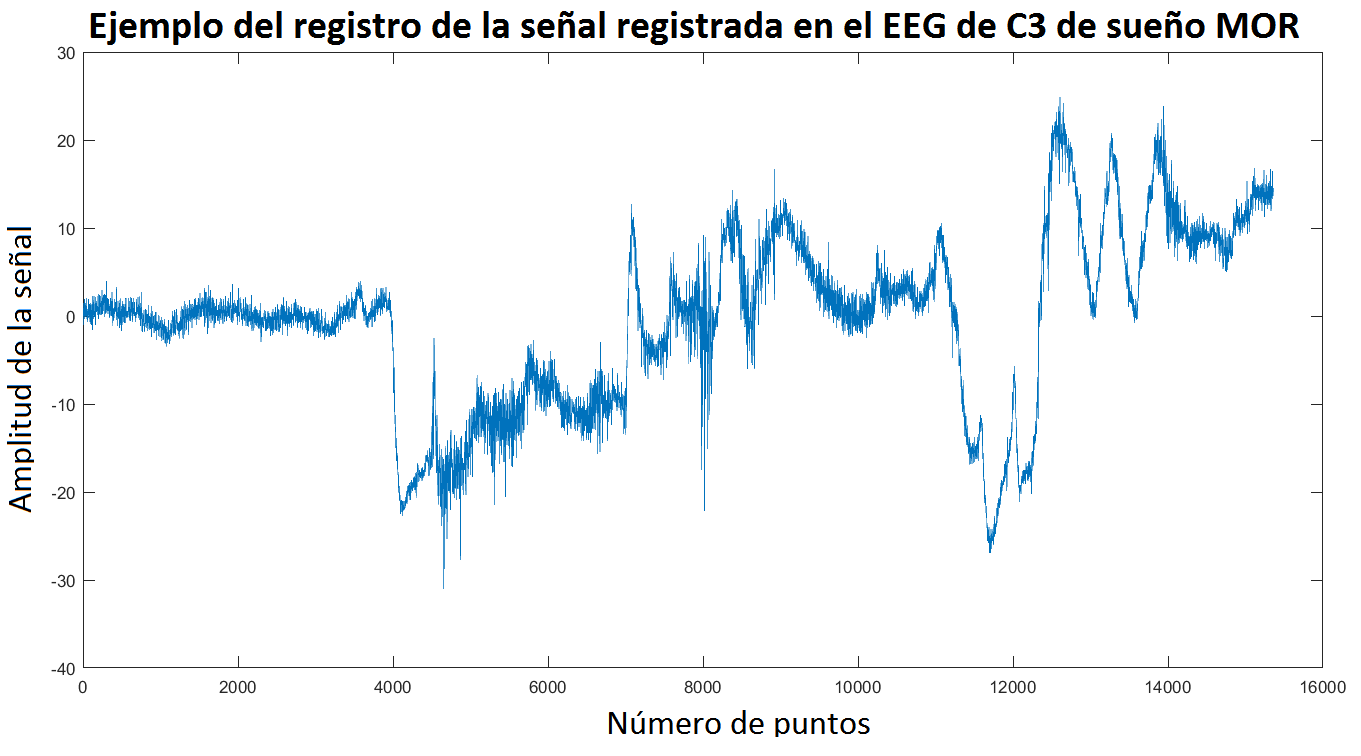
\includegraphics[scale=0.3]{Ejemplo.png}
\caption{Gr\'afico de los datos obtenidos del canal C3 en la \'epoca de sue\~no MOR de un adulto mayor sin deterioro cognitivo.}
\label{ejemplo}
\end{center}
\end{figure}

Primero es necesario saber el tama\~no que tendr\'an las ventanas que dividir\'an a la serie original, en este caso vamos a considerar que el tama\~no de ventana sea de 3350 puntos, teniendo un total de 4 ventanas, es decir, 13,400 puntos en total. Notemos que no se estan considerando todos los puntos de la serie original, ya que en caso de considerar una quinta ventana, esta no estar\'ia completa.\\

Sea a serie de tiempo $x(i)=1,2,3,...,13400$, calculamos el promedio de los 13400 puntos y se tiene $\displaystyle \hat{x}=\frac{1}{13400} \sum_{i=1}^{13400} x(i)=-2.0891$. Calculamos la nueva serie de tiempo $y(k)$ \eqref{st_integrada}.\\

\begin{table}[]
\centering
\caption{Ecuaciones para obtener la serie $y(k)$}
\begin{tiny}
\begin{tabular}{ll}
\hline
$k$      & $y(k)$                                                                                \\
\hline
1        & $\displaystyle y(1)=\sum_{i=1}^{1}(x(i)-(-2.0891))=0.9-(-2.0891)=2.9891$                            \\
2        & $\displaystyle y(2)=\sum_{i=1}^{2}(x(i)-(-2.0891))=y(1)+(-0.4+(-2.0891))=4.6782$                    \\
3        & $\displaystyle y(3)=\sum_{i=1}^{3}(x(i)-(-2.0891))=y(2)+(-1+(-2.0891))=5.7673$                      \\
$\vdots$ & \multicolumn{1}{c}{$\vdots$}                                                          \\
13400    & $\displaystyle y(13400)=\sum_{i=1}^{13400}(x(i)-(-2.0891))
=y(13399)+(9.2+(-2.0891))=0.000000000454$\\
\hline
\end{tabular}
\end{tiny}
\label{tabla}
\end{table}

Una vez que se obtienen los puntos de $y(k)$, se puede apreciar en el siguiente gr\'afico \ref{ejemplo1}:

\begin{figure}[H]
\begin{center}
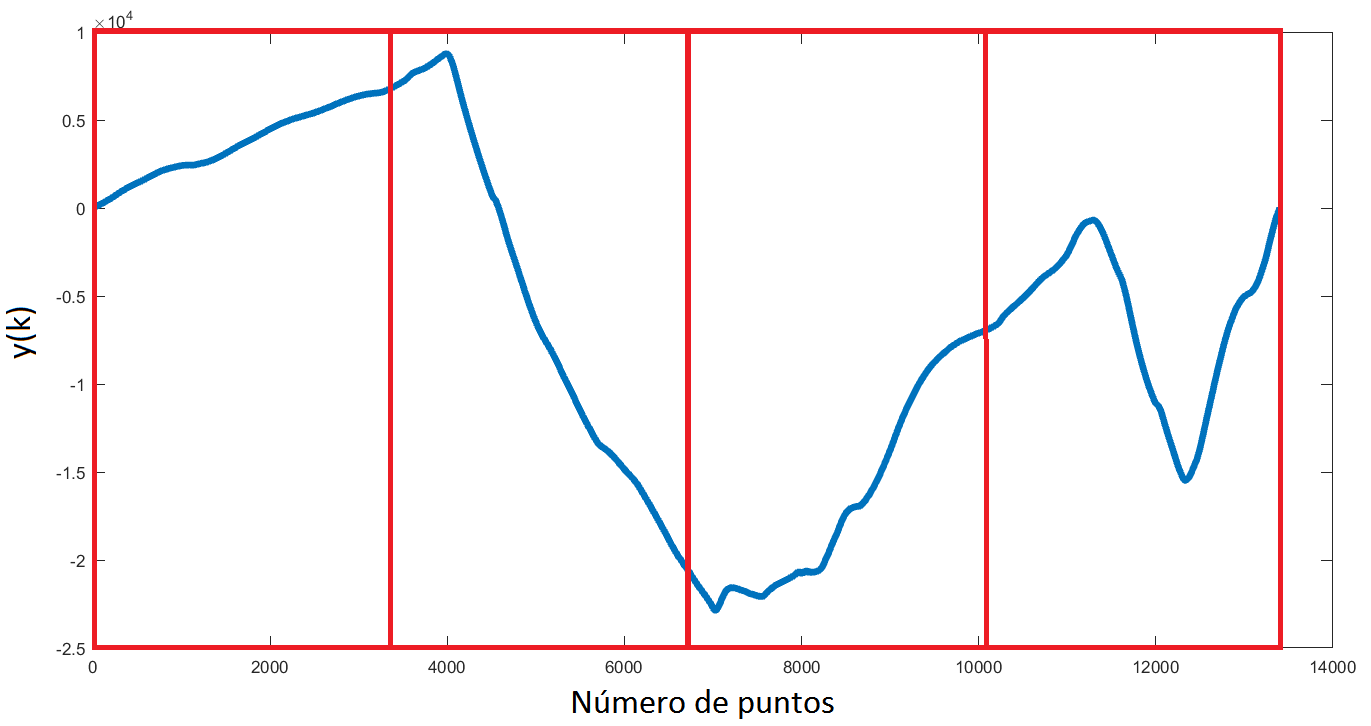
\includegraphics[scale=0.35]{ejemplointegrada1.png}
%Falta agrergar las lineas obtenidas por minimos cuadrados.
\caption{Representaci\'on de la separaci\'on de las ventanas de tama\~no 3350 de la serie intgrada $y(k)$. \ref{ejemplo}}
\label{ejemplo1}
\end{center}
\end{figure}

Para quitar la tendencia lineal local de cada ventana se realiza un ajuste lineal por m\'inimos cuadrados.\\ 

Se denota al valor de la coordenada $y$ de la l\'inea recta como $y_{4}(k)$. Para quitar la tendencia lineal de $y(k)$ se sustrae la tendencia local lineal $y_{4}(k)$. De lo anterior se tiene:

\begin{equation*}
\begin{split}
F(3350) & =\sqrt{\frac{1}{13400}\sum_{i=1}^{13400}(y(i)-y_4(k))^2}\\
& \quad =\sqrt{4813494,01815568}\\
& \quad =2193,96764291447
\end{split}
\end{equation*}



Este paso se repite para ventanas de 6 puntos hasta 9494 puntos. Una vez que tenemos tales resultados, procedemos a registrarlos en un tabla, para posteriormente realizar la escala logar\'itmica del tama\~no de la ventana con respecto a la fluctuaci\'on que se obtuvo \ref{tablalog}.

\begin{table}[H]
\centering
\caption{Datos obtenidos del tama\~no de las ventanas y la fluctuaci\'on correspondiente. As\'i como su escala logar\'itmica}
\label{tablalog}
\begin{tiny}
\resizebox{\textwidth}{!}{%
\begin{tabular}{|
>{\columncolor[HTML]{FFFFC7}}l |l|l|l|
>{\columncolor[HTML]{FFFFC7}}l |l|l|l|}
\hline
\multicolumn{1}{|c|}{\cellcolor[HTML]{FFCE93}n} & \multicolumn{1}{c|}{\cellcolor[HTML]{FFCE93}Fn} & \multicolumn{1}{c|}{\cellcolor[HTML]{FFCE93}log(n)} & \multicolumn{1}{c|}{\cellcolor[HTML]{FFCE93}log(Fn)} & \multicolumn{1}{c|}{\cellcolor[HTML]{FFCE93}n} & \multicolumn{1}{c|}{\cellcolor[HTML]{FFCE93}Fn} & \multicolumn{1}{c|}{\cellcolor[HTML]{FFCE93}log(n)} & \multicolumn{1}{c|}{\cellcolor[HTML]{FFCE93}log(Fn)} \\ \hline
6 & 0,3410 & 0,7782 & -0,4673 & 272 & 32,7163 & 2,4346 & 1,5148 \\ \hline
7 & 0,4688 & 0,8451 & -0,3290 & 296 & 44,7784 & 2,4713 & 1,6511 \\ \hline
8 & 0,5954 & 0,9031 & -0,2252 & 323 & 43,3917 & 2,5092 & 1,6374 \\ \hline
9 & 0,7126 & 0,9542 & -0,1471 & 352 & 52,8627 & 2,5465 & 1,7231 \\ \hline
10 & 0,8153 & 1,0000 & -0,0887 & 384 & 70,8892 & 2,5843 & 1,8506 \\ \hline
11 & 0,9014 & 1,0414 & -0,0451 & 419 & 74,4249 & 2,6222 & 1,8717 \\ \hline
12 & 1,0333 & 1,0792 & 0,0142 & 457 & 97,3706 & 2,6599 & 1,9884 \\ \hline
13 & 1,1791 & 1,1139 & 0,0716 & 498 & 102,1631 & 2,6972 & 2,0093 \\ \hline
14 & 1,2940 & 1,1461 & 0,1119 & 543 & 143,0328 & 2,7348 & 2,1554 \\ \hline
16 & 1,4535 & 1,2041 & 0,1624 & 592 & 153,4498 & 2,7723 & 2,1860 \\ \hline
17 & 1,5668 & 1,2304 & 0,1950 & 645 & 183,7535 & 2,8096 & 2,2642 \\ \hline
19 & 1,7972 & 1,2788 & 0,2546 & 704 & 194,0914 & 2,8476 & 2,2880 \\ \hline
20 & 1,8415 & 1,3010 & 0,2652 & 768 & 229,6352 & 2,8854 & 2,3610 \\ \hline
22 & 2,1198 & 1,3424 & 0,3263 & 838 & 273,3345 & 2,9232 & 2,4367 \\ \hline
24 & 2,3055 & 1,3802 & 0,3628 & 913 & 268,1394 & 2,9605 & 2,4284 \\ \hline
26 & 2,3492 & 1,4150 & 0,3709 & 996 & 288,2378 & 2,9983 & 2,4598 \\ \hline
29 & 2,6030 & 1,4624 & 0,4155 & 1086 & 398,2359 & 3,0358 & 2,6001 \\ \hline
31 & 2,7657 & 1,4914 & 0,4418 & 1184 & 419,9217 & 3,0734 & 2,6232 \\ \hline
34 & 2,9859 & 1,5315 & 0,4751 & 1292 & 408,4695 & 3,1113 & 2,6112 \\ \hline
37 & 3,1225 & 1,5682 & 0,4945 & 1409 & 520,8524 & 3,1489 & 2,7167 \\ \hline
40 & 3,3003 & 1,6021 & 0,5185 & 1536 & 455,9131 & 3,1864 & 2,6589 \\ \hline
44 & 3,5138 & 1,6435 & 0,5458 & 1675 & 726,4486 & 3,2240 & 2,8612 \\ \hline
48 & 3,7020 & 1,6812 & 0,5684 & 1827 & 971,6796 & 3,2617 & 2,9875 \\ \hline
52 & 3,8923 & 1,7160 & 0,5902 & 1992 & 828,6775 & 3,2993 & 2,9184 \\ \hline
57 & 4,2202 & 1,7559 & 0,6253 & 2172 & 1194,7214 & 3,3369 & 3,0773 \\ \hline
62 & 4,0091 & 1,7924 & 0,6030 & 2369 & 1053,5310 & 3,3746 & 3,0226 \\ \hline
68 & 4,8110 & 1,8325 & 0,6822 & 2583 & 1625,1189 & 3,4121 & 3,2109 \\ \hline
74 & 4,9322 & 1,8692 & 0,6930 & 2817 & 1252,1294 & 3,4498 & 3,0976 \\ \hline
81 & 5,6484 & 1,9085 & 0,7519 & 3072 & 1237,9050 & 3,4874 & 3,0927 \\ \hline
88 & 6,1113 & 1,9445 & 0,7861 & {\color[HTML]{FE0000} 3350} & {\color[HTML]{FE0000} 2193,9676} & {\color[HTML]{FE0000} 3,5250} & {\color[HTML]{FE0000} 3,3412} \\ \hline
96 & 5,8498 & 1,9823 & 0,7671 & 3653 & 1501,8246 & 3,5626 & 3,1766 \\ \hline
105 & 7,3770 & 2,0212 & 0,8679 & 3864 & 629,9272 & 3,5870 & 2,7993 \\ \hline
114 & 7,8249 & 2,0569 & 0,8935 & 4344 & 1846,5948 & 3,6379 & 3,2664 \\ \hline
124 & 9,5595 & 2,0934 & 0,9804 & 4708 & 2651,8729 & 3,6728 & 3,4236 \\ \hline
136 & 10,2739 & 2,1335 & 1,0117 & 5166 & 1838,2147 & 3,7132 & 3,2644 \\ \hline
148 & 10,8933 & 2,1703 & 1,0372 & 5634 & 2236,2678 & 3,7508 & 3,3495 \\ \hline
161 & 13,5273 & 2,2068 & 1,1312 & 6144 & 3190,2805 & 3,7885 & 3,5038 \\ \hline
176 & 13,7475 & 2,2455 & 1,1382 & 6700 & 2993,9076 & 3,8261 & 3,4762 \\ \hline
191 & 16,9589 & 2,2810 & 1,2294 & 7306 & 3947,2793 & 3,8637 & 3,5963 \\ \hline
209 & 23,1499 & 2,3201 & 1,3645 & 7968 & 3414,3127 & 3,9013 & 3,5333 \\ \hline
228 & 22,4216 & 2,3579 & 1,3507 & 8689 & 4691,7909 & 3,9390 & 3,6713 \\ \hline
249 & 34,2265 & 2,3962 & 1,5344 & 9474 & 6141,7400 & 3,9765 & 3,7883 \\ \hline
\end{tabular}%
}
\end{tiny}
\end{table}

Una vez obtenidos los valores de la variable dependiente $Fn$ dado el tama\~no de la ventana $n$, los valores se representan con una doble escala logar\'itmica ($\log Fn$,$\log n$), como se muestran en la figura \ref{ejem1}.

\begin{figure}[H]
\begin{center}
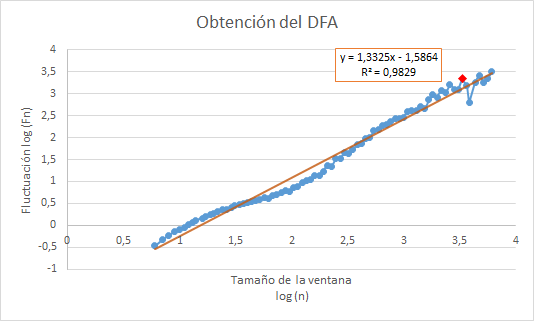
\includegraphics[scale=1]{ejem2.png}
\caption{Representaci\'on de la doble escala logar\'itmica $\log Fn$ vs $\log n$, representada de color azul, donde se resalta de color rojo al tama\~no de ventana 3350, el cual ayudo para ilustrar el m\'etodo DFA. Mostrando a su vez la l\'inea de tendencia correspondiente al mismo, de color naranja, as\'i como la ecuaci\'on de la misma, para poder apreciar el valor de su pendiente, es decir, el par\'ametro de autosimilitud $\alpha$.}
\label{ejem1}
\end{center}
\end{figure}

Posteriormente, se obtiene la l\'inea de tendencia de tal gr\'afico, cuya ecuaci\'n nos permite conocer el par\'ametro de autosimilitud $\alpha$, siendo $\alpha$ representado como la pendiente de la misma.\\

De esta manera de obtiene el valor de autosimilud de una \'epoca de sue\~no MOR, el cual posteriormente se compara con los valores de autocorrelaci\'on establecidos en el la secci\'on del An\'alisis de Fluctuaci\'on sin Tendencia (DFA). En este caso el valor es 1.256, acercandose al par\'ametro $\alpha=1$, ruido rosa. 

\end{document}